%\documentclass{article}
%\usepackage{amssymb}
%\usepackage{wasysym}
%\usepackage{graphicx}
%\usepackage{bm}
%\usepackage{psfig}
%\newcommand{\bc}{\begin{center}}
%\newcommand{\ec}{\end{center}}
%\newcommand{\be}{\begin{equation}}
%\newcommand{\ee}{\end{equation}}
%\newcommand{\bea}[1]{\begin{eqnarray}\label{#1}}
%\newcommand{\eea}{\end{eqnarray}}
%\newcommand{\bua}{\begin{eqnarray*}}
%\newcommand{\eua}{\end{eqnarray*}}
%\newcommand{\infint}{\int_{-\infty}^{\infty}}
%\newcommand{\dd}[2]{{{d#1}\over{d#2}}}
%\newcommand{\ddt}[1]{\dd{#1}{t}}
%\newcommand{\dddt}[1]{\dd{^2#1}{t^2}}
%\newcommand{\aver}[1]{\langle{#1}\rangle}
%\def\cl#1{{\cal #1}}               % for caligrafic letters
%\def\labs{\mid\!}
%\def\rabs{\!\mid}
%\begin{document}
%\setcounter{section}{7} No need when merging
\chapter{Radio, EUV and X-ray telescopes}

\section{Radio and microwave detection}

Karl Jansky was the first person who observed the galaxy with radio waves in 
1931, thereby discovering Sagittarius A, which marks the massive black hole 
at the center of the Milky Way\footnote{Jansky was actually hired by
  Bell Telephone Labarotories to study the effects of thunderstorms on
  radio frequency communication. He designed an antenna that responded
  to waves at 14.6~m. He found signals from thunderstorms but also
  ``... a steady hiss type static of unknown origing''. The source
  appeared 4 minutes earlier every day, and Jansky concluded that it
  must have a origin outside the solar system, finally identifying the
  source as Milky Way in 1933.}Thus, radio astronomy is the 
oldest of the `new' astronomies. The reason
that radio astronomy was early is in part because radio waves easily penetrate
to ground level; for wavelengths from about 10~mm to 10~m the atmosphere is
almost completely transparent. The absorption becomes almost total at 
$0.5$~mm and between $0.5$~mm and 10~mm there are a number of absorption bands
that are mainly due to oxygen and water vapor. The scale height for H$_2$O 
in the atmosphere is about 2000~m so that observing from high altitudes 
reduces the short wave absorption considerably. Radiation with $\lambda>50$~m
does not penetrate to the ground, because of reflection by the ionosphere.

\begin{figure}[h]
  \centering
%	\psfig{file=jansky-antenna.eps,width=0.7\textwidth}
	\includegraphics[width=0.7\textwidth]{jansky-antenna.eps}
  \caption{Karl Jansky and his antenna.}
  \label{fig:jansky-antenna}
\end{figure}

The unit of intensity that is commonly used in radio astronomy is the 
jansky (Jy)
\[
1~{\rm Jy}=10^{-26}~{\rm W m}^{-2}{\rm Hz}^{-1}
\]
and detectable radio sources vary from about $10^{-3}$ to $10^6$~Jy. Most
radio sources generate their flux as thermal radiation, which by the 
Rayleigh-Jeans law gives a spectrum
\[
F_\nu={2\pi k\over c^2}T\nu^2,
\]
or by synchrotron radiation from energetic electrons spiralling around
in magnetic fields, where the spectrum is in the form
\[
F_\nu\propto\nu^{-\alpha},
\]
where $\alpha$ is called the spectral index of the source, and is related
to the energy distribution of the electrons. For most sources it is in the
range $0.2\le \alpha\le 1.2$.

\section{Detectors and receivers}

The detection of radio signals is a two-stage process in which the sensor
produces an electrical signal that then has to be processed until it is in
a usable form. In the MHz radio region, the sensor is normally a dipole 
placed at the focus of a telescope, such as a half-wave dipole. The two halves
of such a dipole are each a quarter of a wavelength long. 

In the GHz and higher frequencies a horn antenna is normally used to collect 
the radiation, usually with waveguides for the connection to the rest of the 
system, though plastic and quartz lenses may be used at very high frequencies.
The sensor at the higher frequencies is normally a 
superconductor-insulator-superconductor (SIS) device. In an SIS detector, an
electron in one superconducting film absorbs film absorbs a photon, giving the
electron enough energy to tunnel through the insulating barrier into the other
superconducting film. This process, known as photon-assisted tunneling, 
produces one electron for every absorbed photon. Devices are based upon two
niobium layers separated by an insulating region of aluminium oxide around
1~nm thick and the whole cooled to 4~K or less.

The signal from the sensor is carried to the receiver whose purpose is 
to convert the high frequency electrical currents into a convenient form.
The behaviour of the receiver is governed by five parameters: sensitivity,
amplification, bandwidth, receiver noise level, and integration time. The
sensitivity and the other parameters are very closed linked, for the minimum
detectable brightness, $B_{\rm min}$, is given by
\[
B_{\rm min}={2k\nu^2KT_s\over c^2\sqrt{t\Delta\nu}}
\]
where $T_s$ is the noise temperature of the system, $t$ is the integration 
time, $\Delta\nu$ is the frequency bandwidth and $K$ is a constant close to 
unity that is a function of the type of receiver. The receiver noise originates
as thermal noise within the electrical components of the receiver, and may also
be called Johnson or Nyquist noise. It is usually necessary to cool the initial
stages of the receiver with liquid helium in order to reduce $T_s$ to an 
acceptable level.


\begin{figure}[h]
  \centering
%	\psfig{file=heterodyne.eps,width=0.95\textwidth}
	\includegraphics[width=0.95\textwidth]{heterodyne.eps}
  \caption{Block diagram of a basic heterodyne receiver (figure adapted from Kitchin {\it
Astrophysical Techniques}).}
  \label{fig:heterodyne}
\end{figure}


\paragraph{Heterodyne receiver.}  
In figure~\ref{fig:heterodyne} we show schematically the set up for a heterodyne receiver. The
pre-amplifier operates at the signal frequency and will typically have a gain of 10 to 1000. The
local oscillator produces a signal that is close to but different from the main signal in its 
frequency. Thus when the mixer combines the main signal and the local oscillator, the beat 
frequency between them (intermediate frequency or IF) is at a much lower frequency than that of
the original. The relationship between them is 
\[
\nu_{\rm signal}=\nu_{\rm LO}\pm\nu_{\rm IF}.
\]
Normally, at lower frequencies only one of the two possible frequencies will be picked up by 
the feed antenna or passed by the pre-amplifier. The power of the IF emerging from the mixer
is directly proportional to the power of the original signal. The IF amplifiers and filter 
determine the pre-detector bandwidth of the signal and further amplify it by a factor $10^6$ to
$10^9$. In the final stages of the receiver, the signal from the detector is integrated, usually for
a few seconds, to reduce the noise level. Then it is fed to an output device, usually 
analogue-to-digital input to a computer for further processing.

The basic heterodyne system has a high system temperature and unstable gain.
The temperature can be lowered by applying an equal and opposite voltage in the
later stages of the receiver, and the stability of the gain can be improved by
switching rapidly from the antenna to a calibration noise source and back again, 
with a phase sensitive detector to correlate the changes. Such a system is called 
a Dicke radiometer. The radiometer work optimally if the calibration noise source
has the same temperature as the signal. The value of $T_s$ varies from 10~K at 
1~m to $10\,000$~K at 1~mm. At long wavelengths diodes can be used as noise 
sources, while at short wavelenghts gas discharge tubes can be used.

Receivers are generally sky background limited. The Earth's atmosphere 
radiates at 100~K and higher temperatures below a wavelength of about
3~mm. Only between 30 and 100~mm does its temperature fall as low as 
2~K. At longer wavelengths, the galactic emission becomes important, rising
to $10^5$~K at wavelengths of 30~m.

Spectrographs at radio frequencies can be obtained in several different ways. 
Today, most radio spectroscopy is carried out by auto-correlation. Successive
delays are fed into the signal that is then cross-correlated with the original
signal in a computer. The spectrum is obtained from the Fourier transform
of the result. Note that this technique is very similar to the Fourier
transform spectrometers to be discussed later.

Alternately the radio signal mey be converted into a different type of
wave, and the variations in this secondary wave studied instead. This
is the principle behind the {\it acousto-optical radio spectrometer} (AOS).

A major problem at all frequencies in radio astronomy is interference from
artificial sources. In theory, certain regions of the spectrum are reserved
partially or exclusively for use by radio astronomers, but leakage from
devices such as microwave ovens, incorrectly tuned receivers, and illegal 
transmissions often overlap these bands. For example the Russian GLONASS
satellite navigation system overlaps into the band reserved for interstellar
OH lines at 1.61~GHz.

\section{Radio telescopes} % Changed from capital T to small t.

The nature of electro-magnetic radiation is the same whether it be radio waves
or optical light that is discussed. On the other hand, the image in an optical 
telescope is discussed in terms of its diffraction structure, while that of 
a radio telescope is discussed in terms of its polar diagram. However, these 
are just two different approaches to the presentation of the same information.
The polar diagram is a plot, in polar coordinates, of the sensitivity or 
voltage output of the telescope, with the angle of the source from the
optical axis (note that we are discussing sources that are far from the 
receiver). The polar diagram may be physically realized by sweeping the 
telescope past a point source, or by using the telescope as a transmitter
and measuring the signal strength around it.

The polar diagram, and hence the performance of the antenna, may be described
by four parameters: the beam width at half-power points (BWHP), the 
beam width at first nulls (BWFN), the gain, and the effective area. The first
nulls are the positions on either side of the optical axis where the 
sensitivity of the antenna first decreases to zero. Thus, the value of the 
BWFN for the half-wave dipole is 180$^{\circ}$. The first nulls are the direct 
equivalent of the first fringe minima in the diffraction pattern of an optical
image, and for a dish antenna type of radio telescope, their position is given
by 
\[
{\rm BWFN}=2\times{1.22\lambda\over D}
\]
The half power points may be best understood by regarding the radio telescope
as a transmitter; they are then the directions in which the broadcast power
has fallen to one half of its peak value. The maximum gain or directivity
is also best understood in terms of a transmitter. It is the ratio of the 
peak value of the output power to the average power. The effective area of 
an antenna is the ratio of its output power to the strength of the incoming
flux of the radiation that is correctly polarized to be detected by the antenna
\[
A_{\rm e}={P_\nu\over F_\nu}
\]
where $A_{\rm e}$ is the effective area, $P_\nu$ is the power output by the 
antenna at frequency $\nu$ and $F_\nu$ is the correctly polarized flux from the
source at the antenna at frequency $\nu$. The effective area and maximum gain
$g$ are related by 
\[
g={4\pi\over c^2}\nu^2A_{\rm e}.
\]
For the half-wave dipole, the maximum gain is about 1.6, and so there is very
little advantage over an isotropic receiver. 

\begin{figure}[h]
  \centering
%	\psfig{file=polar_plot.eps,width=0.95\textwidth}
	\includegraphics[width=0.95\textwidth]{polar_plot.eps}
  \caption{Polar plots for a single half-wave dipole, collinear arrays with two and four 
dipoles and an isotropic receiver.}
  \label{fig:polar_plot}
\end{figure}

The performance of a simple dipole may be improved by combining the 
outputs from several dipoles that are arranged in an array. In a co-linear 
array, the dipoles are lined up along their axes and spaced at intervals
of half a wavelength. The arrangement is equivalent to a diffraction
grating and so the sensitivity at an angle $\theta$ to the Long axis
of the array $s(\theta)$ is given by
\[
s(\theta)=s_0\left({\sin(n\pi\sin\theta)\over\sin(\pi\sin\theta)}\right)
\]
where $n$ is the number of half-wave dipoles and $s_0$ is the gain of a single
half wave dipole which is $\propto \cos^2\theta$. 
Examples of polar diagrams are shown in figure~\ref{fig:polar_plot}.
The resolution along the axis of the array, measured to the
first null is 
\[
\alpha=\sin^{-1}\left(1\over n\right).
\]
Although the resolution of an array is improved over that of a simple dipole along 
its optical axis, it will still accept radiation form any point perpendicular to the array
axis. The use of a {\it broadside array} in which the dipoles are perpendicular to the 
array axis and spaced at half wavelength intervals can limit the acceptance angle. 

Even so there is a twofold ambiguity in direction of a source that has been detected. 
This can be removed by placing a reflector behind the dipole. This is simply a conducting rod 
about 5\% longer than the dipolse and unconnected electrically with it. It
is placed parallel to the dipole and about one eighth of a wavelength behind
it. For an array, the reflector may be a similarly placed electrically 
conducting screen. Such a reflector is termed a {\it parasitic element} since it is not part 
of the electrical circuit of the antenna. Similar parasitic elements may be added in front 
the dipole to act as directors.

With a reflector and several directors we obtain the parasitic or {\it Yagi} antenna, perhaps 
familiar from its appearance on rooftops as a television antenna. The main use of parasitic
antenna in radio astronomy is as the receiving element of a larger reflector such as a parabolic
dish.

The use of a single dipole, or even several dipoles in an array, is the
radio astronomy equivalent of naked-eye observation. The most usual method
of concentrating the signal is to construct large parabolic dishes. These
are directly equivalent to an optical reflecting telescope.They are
usually used at the prime focus or at the Cassegrain focus. The gain may 
be found roughly by substituting the dishes' area for the effective area. 
The size of telescopes is so large because of the length of the wavelength
being observed. The requirement on surface accuracy is the same as that for
an optical telescope: deviations from the paraboloid must be less than 
$\lambda/8$ if the Rayleigh resolution is not to be degraded, in practice a
limit of $\lambda/20$ is often used. Note also that the surface of the 
``mirror'' need not be solid, a wire mesh with spacings less than $\lambda/20$
will function equally well as a reflector. This has large implications for the
weight and wind resistance of the dish. The dishes are usually of very 
small focal ratios (f0.5 or so) and the reason is so that the dish acts
as a screen against unwanted radiation. Fully steerable dishes up to 100~m
across have been built, while the Arecibo telescope is a fixed dish 300~m 
across. In the microwave region the largest dishes are currently the 30~m IRAM
instrument on Pico Veleta in Spain and the 45~m telescope at Nobeyama in Japan.

With a single feed, the radio telescope is a point source detector only. 
Images have to be built up by scanning or by interferometry. 

True imaging can be achieved by the use of cluster or array feeds. 
These are simply multiple individual feeds arranged in a suitable array at
the telescope's focus. Each feed is then the equivalent of a pixel in a CCD.
The number of elements in such cluster feeds currently remains small compared
to their optical equivalents; for example the 64~m Parkes radio telescope
uses a 13-beam receiver for 21~cm radiation. 

Very many other systems have been designed to fulfill the same function as
a steerable paraboloid but which are easier to construct. 

Another approach is used in the Mills Cross type telescope. This uses
two perpendicularly oriented collinear arrays, {\it e.g.} 
north--south and east--west. The first provides a
narrow fan beam along the north--south direction while the second provides a similar 
beam in the east--west direction. Their intersection is a narrow vertical pencil beam, 
typically $1^{\circ}$ across. This beam can be isolated from the contributions of the 
remainder of the fan beams by comparing the outputs when the beams are added 
in phase and when they are added out of phase. This pencil beam can be displaced
an angle $\theta$ from the vertical by introducing a phase shift between each dipole.

Yet another approach is based on refraction. The Luneburg lens is a solid sphere 
within which the refractive index increases linearly inward from unity at the surface.
With a central refractive index of 2, the focus is on the surface of the lens. Since there
is no axis of symmetry, the lens can be used to observe in many directions simultaneously,
simply by having many feeds distributed around it. The Luneburg lens has yet to 
find application in radio astronomy, but may be used in the Square Kilometer Array.

\paragraph{Spacecraft.} A number of spacecraft carrying microwave detectors have been launched. 
These include COBE, MAP and Planck which all are designed to measure anisotropies in
 the cosmic microwave background radiation.

\subsection{Construction}

Largest problem is wind: {\it e.g.} up to $1.5\times 10^6$~N for a 50~m dish 
facing directly into a gale-force wind. There are only two solutions to the wind problem:
to enclose the dish, or to cease using it when the wind load becomes too great. Some 
smaller dishes are therefor enclosed in {\it radomes}, which are space-enclosing structures
built from non-conducting materials.

\section{X-ray and gamma-ray detection}

This third region of the spectrum to be discussed is the most recent area
to be explored. None of the radiation penetrates to ground level, so its
study had to await the availability of observing platforms in space, or near
the top of the Earth's atmosphere. The high energy spectrum can be divided into
\begin{itemize}
\item extreme ultraviolet (EUV): 10 to 100~nm (12 to 120~eV)
\item soft x-rays: 1 to 10~nm (120 to 1200~eV)
\item x-rays: $0.01$~nm 1~nm (1.2 to 120~keV)
\item soft gamma-rays: $0.001$ to $0.01$~nm (120 to 1200~keV)
\item gamma-rays: less than $0.001$~nm (greater than 1.2~MeV)
\end{itemize}

The main production mechanisms for high-energy radiation include electron
synchrotron radiation, the inverse Compton effect, free-free radiation, 
and pion decay, while the sources include the Sun, supernova remnants, pulsars,
bursters, binary systems, cosmic rays, the intergalactic medium, galaxies,
Seyfert galaxies, and quasars. The interstellar absorption in this region
varies roughly with the cube of the wavelength, so that the highest 
energy radiation can easily pass through the whole galaxy with little 
chance of being intercepted. The flux of radiation varies enormously
with wavelength. The solar emission alone at the lower energies is 
sufficient to produce the ionosphere and thermosphere on the Earth. At 
1~nm wavelength, for example, the solar flux is 
$5\times 10^9$~photons$\,$m$^{-2}$s$^{-1}$, while the total flux from all sources
above $10^9$~eV is only a few photons per square meter per day.

\subsection{Detectors}

\paragraph{Geiger counters.} Two electrodes inside an enclosure are held at such a 
potential difference that a discharge in the medium filling the enclosure
is on the point of occurring. The medium inside the tube is typically argon at a 
low pressure with a small amount of organic gas, such as alcohol vapour added.
The entry of ionizing radiation triggers this discharge,
resulting in pulse of current between the electrodes that then may be amplified and
detected. The electrons produced in the initial ionization are accelerated towards
the central electrode by the applied potential; as these electrons gain energy they
cause further ionization, producing more electrons, and so on. Gain of some $10^8$ electrons for every one in the initial ionizing trail. The avalanche of electrons rapidly 
saturates, so that the detected pulse is independent of the original energy of the
photon. Another disagvantage of Geiger counters, shared by many of the
detectors described below is that a response to one event leaves the
detector inoperative for a short invterval, known as the dead
time, caused by the reduction in the potential between the
electrodes. The length of the dead time for this type of detector is of
order 200~$\mu$s.

\paragraph{Proportional counters.} Geiger counters run at a lower voltage, so that 
saturation is avoided and the strength of the signal is proportional to the
original signal. The gain is reduced to $10^4$, $10^5$. Provided all the
energy of the ionizing radiation is absorbed withing the detector, its
original total energy may be obtained from the strength of the pulse. 
At high photon energies the detector is limited by the requirement that 
all the energy of the radiation be contained within the detector. To this
end, proportional counters for high-energy detection may have to be made quite
large. About 30~eV is required to produce one ion-electron pair, so that a
1~keV photon produces about 36 electrons, and a 10~keV photon 360 electrons. 
The spectral energy resolution to two and a half standard deviations is 
thus about 40\% at 1~keV and 12\% at 10~keV. The quantum efficiencies 
of the proportional counter approach 100\% for energies up to
50~keV. The position of interaction of the x-ray along the counter may
be obtained through the use of a resitive anode. The pulse is measured
at both ends of the anode and a comparison of the strength and shape
leads to a leads to the position of the discharge along the anode. The
anode wires are typically very thin, 20~$\mu$m across, so the electric
field is most intense very close to the wire, limiting its spread, and
giving a precise position. This concept can be extended to a 2D grid
of anodes to allow imaging. Spatial resolutions of 0.1~nm are
currently possible and this allows the building of {\it
  position-sensitive proportional counters}. Many
gases can be used to fill the detector: argon, methane, xenon, carbon dioxide,
and mixtures thereof. Inert gases are preferred as there is then no possibility
of the loss of energy into the rotation or vibration of the molecules. 

\begin{figure}[h]
  \centering
%	\psfig{file=GLAST_allsky_labeled_HI.eps,width=0.95\textwidth}
	\includegraphics[width=0.95\textwidth]{GLAST_allsky_labeled_HI.eps}
  \caption{First light on the Large Area Telescope on board the Fermi Gamma-ray
Space Telescope. The photons that have made this image have an energy
greater than 1~GeV.}
  \label{fig:glast_allsky}
\end{figure}

\paragraph{Scintillation detectors.} The ionizing photons do not necessarily knock 
out only the outermost electrons from the atom or molecule with which they 
interact. Electrons in lower energy levels may also be removed. When this 
happens a `hole' is left behind into which one of the higher electrons may
drop, with a consequent emission of radiation. This photon can be observed
with a photomultiplier. 
The noise level is high since only about 3\% of the original x-ray energy
is converted into detectable radiation. Sodium iodide or caesium iodide are 
useful for x-ray energies up to several hundred keV, organic scintillators
such as stilbene (C$_{14}$H$_{14}$N$_2$) can be used up to 10~MeV and bismuth
germanate (Bi$_4$Ge$_3$O$_{12}$) for energies up to 30~MeV or more. Organically
doped plastics are also used. Both sodium iodide and bismuth germanate are used
on the burst monitor on board the Fermi Gamma-ray Space Telescope (formerly
GLAST) launched during the spring of 2008, to provide continuous detection
from some few keV to 25~MeV. 

Discrimination of the x-ray's arrival direction can be obtained by using 
sodium iodide and caesium iodide in two superposed layers. The decay time
of the pulses differ between the two compounds so that they may be 
separately identified, and the direction of travel of the photon inferred.
Several gases such as argon, xenon, nitrogen and their mixtures Can also
be used as scintillators, and combined with an optical system to produce
another imaging device.

\paragraph{Gas scintillation proportional counters.} A combination of the two
above types leads to a significant improvement in the low-energy spectral
resolution. Resolution as good as 6\% at 6~keV has been acheived in practice.
The x-ray radiation produces ion-electron pairs in an argon- or xenon-filled
chamber. The electrons are then gently accelerated until they cause 
scintillation of their own in the gas. These scintillations can then be
observed by a conventional scintillation counter system. 

\paragraph{Charge coupled devices.} (CCDs!) are becoming increasingly widely used as 
primary detectors at EUV and x-ray wavelengths. The Chandra spacecraft 
uses CCDs with a 24~$\mu$m pixel size, giving 0.5~arcsec resolution. CCDs
become insensitive to radiation in the blue and ultraviolet because of the 
absorption in the electrode structure on their surfaces. They regain sensitivity at
shorter wavelengths as radiation is able to penetrate the structure
 (at $\lambda<10$~nm or so).

\paragraph{Cerenkov detectors.} X-Ray and gamma radiation interest lies in the detection
of particles produced by the Compton interaction of very high energy photons. These
particles can achieve velocities greater than that of light in the local medium producing
Cerenkov radiation. For example, such particles can be produced high in the atmosphere 
and observed from the ground with telescopes such as CANGAROO-II in Australia or 
MAGIC on La Palma.

\begin{figure}[h]
  \centering
%	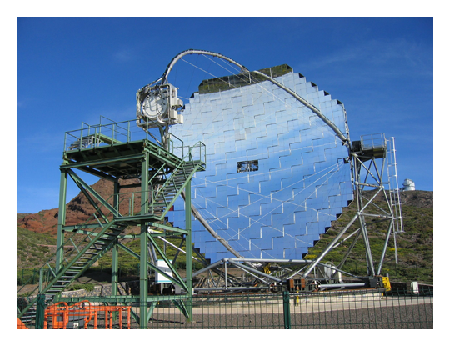
\psfig{file=magic.eps,width=0.7\textwidth}
	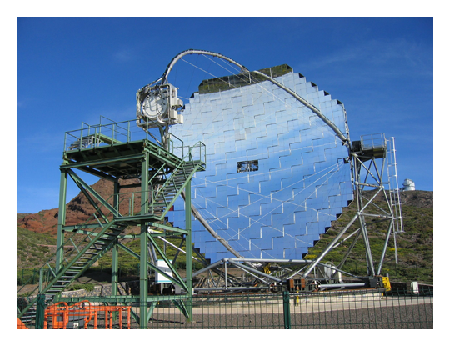
\includegraphics[width=0.7\textwidth]{magic.eps}
  \caption{One of the two (almost) identical MAGIC telescopes on Roque
    de los Muchachos Observatory on La Palma.}
  \label{fig:magic}
\end{figure}                    

\paragraph{Solid-state detectors.} Solid state detectors have several advantages that suit them 
particularly for use in satellite-borne instrumentation> a wide range of photon energies
detected (from 1~keV to 1~MeV), simplicity, reliability, low power consumption, high
stopping power for radiation, room temperature operation, no entrance window needed,
high counting rates, etc. They also have intrinsic spectral sensitivity since, provided the 
photon is absorbed completely, the number of electrons-hole pairs produced is proportional
to the photon's energy. The main disadvantage is that their size is small, so that their 
collecting area is also small, and that unless the photon is stopped within the detector's
volume the total energy cannot be determined. 

INTEGRAL, launched in 2002, carries a spectrometer that uses germanium detectors. In these
a cylinder germanium (cooled by liquid nitrogen) is surrounded by a cylindrical cathode and has
a central anode. A gamma ray scatters off electrons in the atoms until its energy has been
consumed in electron-hole pair production. The number of released electrons is proportional
to the energy of the gamma ray, and these are attracted to the anode where they may be
detected. The spectral resolution is high (0.2\% at 1~MeV) so that detectors of this type
are especially suitable for line spectroscopy. Other materials that may replace germanium
include germanium doped with lithium, cadmium telluride and mercure-iodine. At lower energies
(0.4 -- 4~keV) silicon based  solid-state detectors may be used similarly. Their energy resolution
ranges from 4 -- 30\%.

\paragraph{Microchannel plates.} Microchannel plates are a variant of the photomultiplier. The devices 
are also known as Multi-Anode Micro-channel Arrays (MAMAs). A thin plate is pierced by numerous tiny holes, each perhaps only about 10~$\mu$m across or less. Its top surface is
an electrode with a negative potential of some 1000~V with respect to the base. The top is
coated with a photoelectron emitter for the x-ray energies of interest. An impinging photon
releases one or more electrons that are then accelerated down the tubes. Collisions with the tube
walls will release further electrons, which are in turn accelerated down the tube walls and so on.
As many as $10^4$ electrons can be produced by for a single photon, and this may increased
to $10^6$ electrons in future devices. The quantum efficiency can be up to 20\%. The electrons
spray out of the bottom of each tube, where they may be detected. 

An example is the high resolution x-ray camera aboard Chandra that uses a 93~mm square
chevron microchannel plate detector, with 69 million 10~$\mu$m holes, and can provide a
resolution of 0.5~arcsec. 

Microchannel plates can also be used in the optical and near ultraviolet.

\subsection{Imaging}

\paragraph{Collimation.} A collimator is a device that physically restricts the field of view of the detector
without contributing further any further to the formation of an image. The image is obtained by 
scanning the system across the object. 

The simples arrangement is a series of baffles that may be formed into a variety of configurations. These are generally known as honeycomb collimators, even though the cells are
usually square rather than hexagonal. At high energies, the baffles may be formed from 
a crystal scintillator and pulses from there used to reject detections of radiation from
high inclinations. At the low energies the glancing reflection of the radiation can be used
to produce a truly imaging collimator. This is called a `lobster eye' focusing collimator, 
and is essentially a honeycomb collimator curved into a portion of a sphere with a position 
sensitive detector at its focal surface. 

Another system is known as a modulation collimator
or {\it Fourier transform telescope} uses two or more parallel gratings that are separated by
a short distance. Since the bars of the gratings alternately obscure the radiation and allow it to 
pass through, the output as the system scans a point source is a sine wave. To obtain 
unambiguous positions for the sources, or for the study of multiple or extended sources, 
several such gratings of different resolutions are combined. The image may then be 
retrieved from the Fourier components of the output. Two such grating systems can be
combined at right angles to give a two-dimensional image. 

A third type of system is a simple pinhole camera. A position-sensitive detector is placed 
behind a small aperture. A better system replaces the pinhole with a mask formed from 
clear and opaque regions. The pattern of the mask is known, so that when sources cast 
shadows of it on the detector, their position and structure can be reconstituted in a similar
manner to that used for the modulation collimator. The technique is known as {\it coded 
mask imaging}, and resolutions of 10~arcmin or better can be reached. 

\paragraph{Coincidence detectors.} A telescope, in the sense of being a device with directional sensitivity, may be constructed for use at any energy and with any resolution, by using two
or more detectors in a line, and by rejecting all detections except those which occur in 
both detectors and separated by the correct flight time. Two separated arrays of detectors 
can similarly provide a two-dimensional imaging system.

\paragraph{Occultation.} The occultation of a source by the Moon or other object can be used to 
give very precise positional and structural information.

\paragraph{Reflecting telescopes.} At energies below about 100~keV photons
may be reflected with up to 50\% efficiency off metal surfaces, when
their angle of incidence approaches 90$^o$.

\begin{figure}[h]
  \centering
%	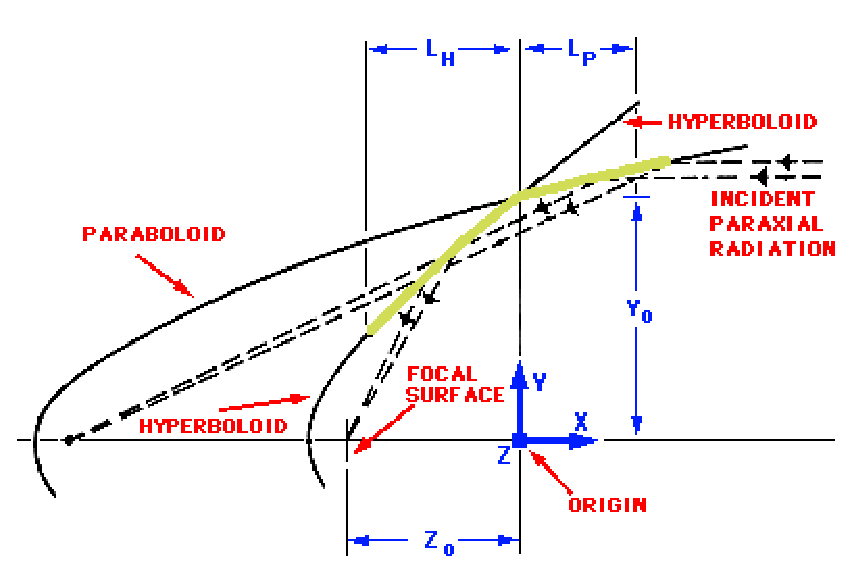
\psfig{file=paraboloid_hyperboloid.eps,width=0.95\textwidth}
	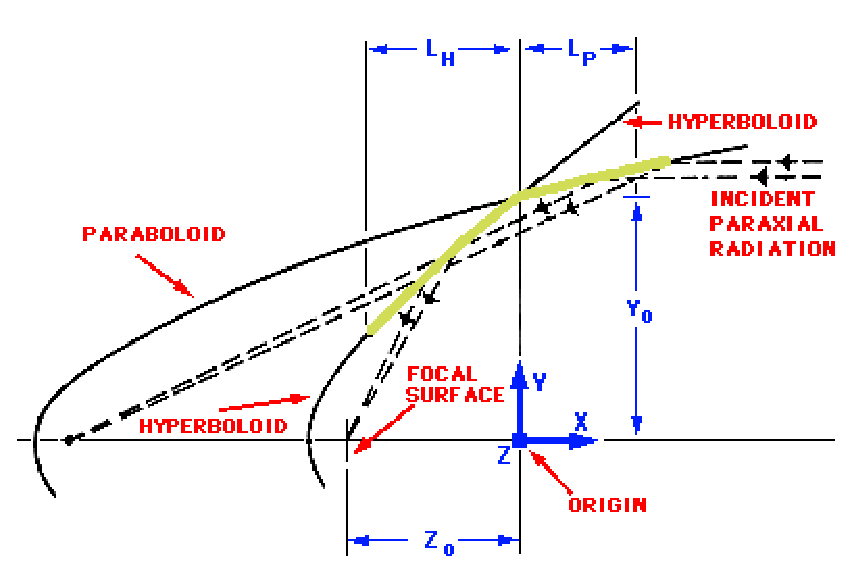
\includegraphics[width=0.95\textwidth]{paraboloid_hyperboloid.eps}
  \caption{Wolther telescope of type {\sc i}.}
  \label{fig:wolther_i}
\end{figure}

Several systems have been devised, but the one which has achieved most practical
use is the is formed from the combination of annular sections of very deep paraboloidal
and hyperboloidal surfaces known as Wolther telescopes. The aperture of such
telescopes is a thin ring, since only the radiation incident on the paraboloid annulus is 
brought to focus. To increase the effective aperture, and hence sensitivity, several
such confocal systems of differing radii may be nested inside each other. For the 
XMM--Newton spacecraft a total of 58 such nested telescope shells gave a total
correcting area of $0.5$~m$^2$. A schematic of a Wolther type {\sc i} telescope is shown
in figure~\ref{fig:wolther_i}.

At lower energies, in the EUV and soft x-ray region, near normal incidence
reflection with efficiencies of up to 20\% is possible using multilayer coatings.
These are formed from tens,  hundreds, or even thousands of alternate layers of 
for example tungsten and carbon, aluminium and gold or magnesium and gold,
each about 1~nm thick. The reflection is essentially monochromatic, with the 
wavelength depending on the orientation of the crystalline structure of the layers and
on their thickness. Reflection of several wavelengths can be achieved by changing 
the thickness of the layers through the stack. The thickest layers are on the top and
reflect the longest, least penetrating wavelengths. Telescopes or relatively 
conventional design are used with these mirrors, and direct images of the Sun 
at wavelengths down to 4~nm can be obtained.

\subsection{Spectroscopy}

Many of the detectors described above are intrinsically capable of separating 
photons of different energies. At photon energies above 10~keV it is only this
inherent spectral resolution which can provide information on the energy spectrum.
Devices akin to the more conventional idea of a spectroscope, however, can only 
be used at the low end of the energy spectrum.

\paragraph{Grating spectrometers.} Gratings may be either transmission or grazing
incidence reflection. The theoretical background for x-ray gratings is identical
to with that for optical gratings (discussed later). Typical transmission
gratings have around $10^3$ lines per mm. The theoretical resolution is
between $10^3$ and $10^4$, but is generally limited in practice to 50 -- 100 by
other aberrations.

Reflection gratings are also similar in design to their optical counterparts.
Their dispersion differs because of the grazing incidence. If the separation
of the rulings is $d$ then the path difference $\Delta P$ of two rays that
are incident on to adjacent rulings is
\[
\Delta P=d[\cos\theta-\cos(\theta+\phi)]
\]
Expanding this to second order we find
\[
\Delta P={1\over 2}d(\phi^2-2\theta\phi).
\]
In the $m$th order spectrum, constructive interference occurs for radiation
of wavelength $\lambda$ if 
\[
m\lambda=\Delta P
\]
so that
\[
\phi=\left({{2m\lambda\over d}+\theta^2}\right)-\theta
\]
and
\[
{d\phi\over d\lambda}=\left({m\over 2d\lambda}\right)^{1/2}
\]
where $\theta^2$ is neglected due to the small size of $\theta$. The
dispersion for a glancing incidence reflection grating is therefore inversely
proportional to the square root of $\lambda$, unlike the case for normal 
incidence, when the dispersion is independent of wavelength.

\paragraph{Bragg spectrometers.} Planes of atoms in a crystal are separated by $0.1$ to 10~nm, which
is comparable to the wavelength of x-rays. Thus, a beam of x-rays interacts with a crystal in 
a complex manner. The details of this interaction was first described by the Braggs. Given
a distance $d$ between crystal planes and an angle of incidence $\theta$ the path difference 
for rays are multiples of the path difference for two adjacent layers
\[ \Delta P=2d\sin\theta \]
There will be constructive interference for path differences that are whole numbers of wavelengths. So the reflected beam will consist of just those wavelengths, $\lambda$, 
for which this is true
\[ m\lambda=2d\sin\theta. \]
A  Bragg spectrometer uses a crystal to produce monochromatic radiation of known wavelength.
When a crystal is illuminated by x-rays of mixed wavelengths, only those fulfilling the requirement above will be reflected. The first order, $m=1$, reflection is by far the strongest.
The whole spectrum can be scanned by tilting the crystal at different angles $\theta$. An improved version of the instrument uses a bent crystal and a collimated beam of x-rays so that 
the approach angle varies over the crystal. The reflected beam then consists of the spectrum at
all wavelengths which can be detected in a single observation with a position sensitive detector. 
Spectral resolutions of up to $10^3$ are possible at 1~keV, but large crystal areas are necessary for good sensitivity.  Among common crystals in use are lithium fluoride, lithium hydride, 
tungsten disulphide, graphite, and potassium acid phthalate. 

%\end{document}
